\section{Model}
\label{section:model-architecture}

\begin{figure}[t]
    \centering
    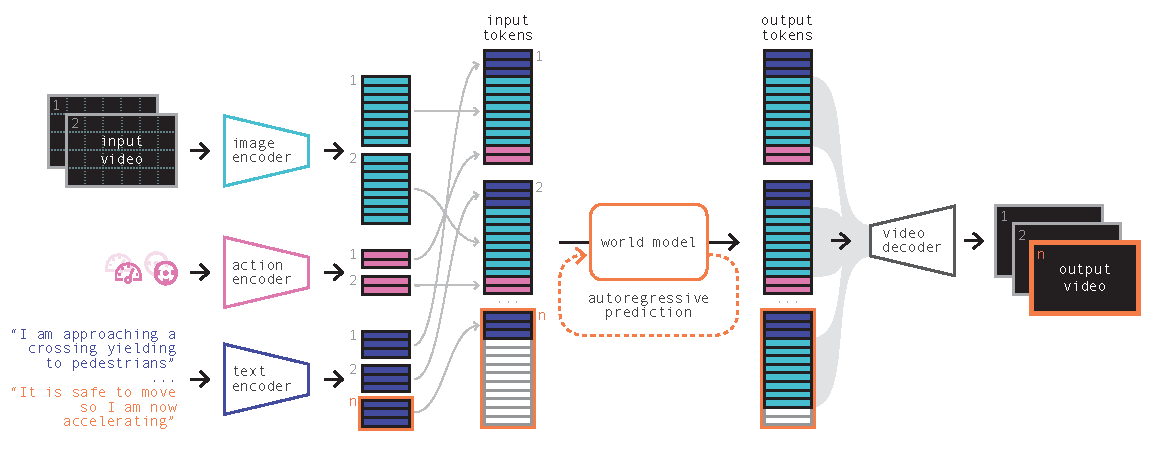
\includegraphics[width=\linewidth]{Figures/Introduction/gaia_schematic.pdf}%
    \caption{Architecture of GAIA-1. First, we encode information from all input modalities (video, text, action) into a common representation: images, text and actions are encoded as a sequence of tokens. The world model is an autoregressive transformer that predicts the next image token conditioned on past image, text, and action tokens. Finally, the video decoder maps the predicted image tokens back to the pixel space, at a higher temporal resolution.} 
    \label{fig:architecture}
\end{figure}

In this section we describe the model architecture of the trainable components of GAIA-1. The general architecture is presented in \Cref{fig:architecture}.

\subsection{Encoding Video, Text and Action}
\label{subsection:encoding}
GAIA-1 can leverage three different input modalities (video, text, action), which are encoded into a shared $d$-dimensional space.

\paragraph{Image tokens.}Each image frame of a video is represented as discrete tokens. To achieve this, we use a pre-trained image tokenizer for discretization (for details about the pre-training see Section~\ref{subsection:image-tokenizer}). Formally, let us consider a sequence of $T$ images $(\rvx_1, \ldots, \rvx_T)$, where each image $\rvx_t$ in this sequence is discretized into $n=576$ discrete tokens using the pre-trained image tokenizer. We obtain a sequence denoted as $(\rvz_1, \ldots, \rvz_T)$, where each $\rvz_t = (z_{t,1}, \ldots, z_{t,n}) \in \mathbb{R}^n$ corresponds to $n = \frac{H}{D} \times \frac{W}{D}$ discrete tokens. Here, $H$ and $W$ represent the height and width of the input image, while $D$ denotes the downsampling factor of the image tokenizer. These discrete tokens are then mapped to a $d$-dimensional space via an embedding layer that is trained alongside the world model. 

\paragraph{Text tokens.} At each time step $t$, we incorporate information from both text and action. Textual input is encoded using the pre-trained T5-large model \citep{2020t5}, resulting in $m=32$ text tokens per time step. These tokens are mapped to a $d$-dimensional space through a linear layer that is trained in conjunction with the world model. This process yields a text representation denoted as $\rvc_t = (\rvc_{t,1}, \ldots, \rvc_{t,m}) \in \mathbb{R}^{m\times d}$.

\paragraph{Action tokens.} For actions, we consider $l=2$ scalar values (representing speed and curvature). Each scalar is independently mapped to the $d$-dimensional space via a linear layer that is trained with the world model. Consequently, the action at time step $t$ is represented as $\rva_t = (\rva_{t,1}, \ldots, \rva_{t,l}) \in \mathbb{R}^{l\times d}$. 

For each time step, the input tokens are interleaved in the following order: text - image - action. The final input of the world model is therefore $(\rvc_1,\rvz_1, \rva_1, \ldots, \rvc_T, \rvz_T, \rva_T)$. To encode the position of the input tokens, we use a factorized spatio-temporal positional embedding. 1) A learnable temporal embedding is shared across all the tokens of a given time step, i.e. there are $T$ temporal embeddings. 2) A learnable spatial embedding indicates the position of a token within a time step, i.e. there are $m + n + l = 610$ spatial embeddings ($m$ text tokens, $n$ image tokens, and $l$ action tokens) of dimension $d=4096$. 


\subsection{Image Tokenizer}
\label{subsection:image-tokenizer}
When modeling discrete input data with a sequence model, there is a trade-off between the sequence length and the vocabulary size. The sequence length refers to the number of discrete tokens that are needed to describe the data. The vocabulary size corresponds to the number of possible values a single token can take. For language, there are two obvious choices for tokens: characters and words. When using character-level tokens, the input data has a longer sequence length, and each individual token belongs to a smaller vocabulary, but conveys little meaning. When using word-level tokens, the input data has a shorter sequence length, and each token contains a lot of semantics but the vocabulary is extremely large. Most language models \citep{roberta19,brown20,2020t5,Chowdhery2022PaLMSL,hoffmann22,llama23} use byte-pair encoding (or equivalent) as a trade-off between character-level and word-level tokenization.

Likewise for video, we would like to reduce the sequence length of the input, while possibly making the vocabulary larger, but with tokens that are more semantically meaningful than raw pixels. We do this with a discrete image autoencoder \citep{oord17}. There are two objectives we would like to achieve in this first stage:

\begin{enumerate}
    \item Compress the information from raw pixels to make the sequence modeling problem tractable. Images contain a lot of redundant and noisy information. We would like to reduce the sequence length needed to describe the input data.
    \item Guide the compression towards meaningful representations, such as semantics, instead of high-frequency signals. The resulting input space for the world model will be simpler to compose with, and less dominated by high-frequency signals that can considerably slow down the learning process.
\end{enumerate}

We reduce the sequence length of the input data by downsampling each input image by a factor $D=16$ in both height and width. Each image $\rvx_t$ of size $H\times W$ is described by $n=\frac{H}{D} \times \frac{W}{D}$ tokens with a vocabulary size $K$. Inspired by~\citep{peng2022beit}, we guide the compression towards meaningful representations by regressing to the latent features of a pre-trained DINO model \citep{caron2021emerging}, a self-supervised image model that is known to contain semantic information. See \Cref{fig:dino_tokenizer} for a qualitative example.

The discrete autoencoder is a fully convolutional 2D U-Net \citep{ronneberger15}. The encoder $E_{\theta}$ quantizes the image features using nearest neighbor look-up from a learnable embedding table \cite{oord17}, resulting in image tokens $\rvz_t = E_{\theta}(\rvx_t)$.  Note that the decoder is only used to train the image autoencoder, solely the discrete encoder $E_{\theta}$ is part of the final GAIA-1 model. Due to the decoder being trained on single images it lacks temporal consistency when decoding to a video. For this reason we also train a video decoder that is described in \Cref{subsection:video-decoder}. 

The training losses for the image autoencoder are the following:
\begin{itemize}
\item \textbf{Image reconstruction loss.} The image reconstruction loss is a weighted sum of $L_1$, $L_2$, perceptual loss $L_{\text{perceptual}}$ \citep{Johnson2016Perceptual}, and GAN loss $L_{\text{GAN}}$ \citep{esser21}.

\item \textbf{Quantization loss.} To update the embedding vectors, we use the embedding loss and the commitment loss from \citep{oord17}. We adopted the linear projection of the embedding and $L_2$ normalization from \citep{yu2022vectorquantized} as we found this helped increase vocabulary usage.

\item \textbf{Inductive bias loss.} The quantized image features are encouraged to match the image features of a pre-trained DINO \citep{caron2021emerging} model with a cosine similarity loss. Distilling the information from DINO into the learned tokens is important as it allows them to benefit from the inductive biases of this model.
\end{itemize}

\begin{figure}[t]
    \centering 
\begin{subfigure}{0.33\textwidth}
  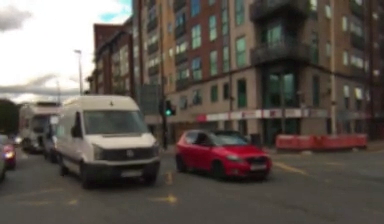
\includegraphics[width=\linewidth]{Figures/Tokenizer/frame1_image.png}
  \caption{Input image}
  \label{fig:tokenizer_a}
\end{subfigure}\hfil 
\begin{subfigure}{0.33\textwidth}
  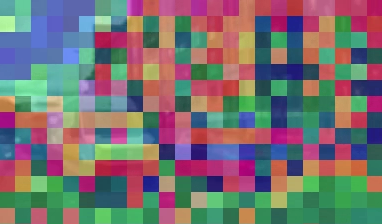
\includegraphics[width=\linewidth]{Figures/Tokenizer/frame1_vqgan.png}
  \caption{Base VQ-GAN tokens}
  \label{fig:tokenizer_b}
\end{subfigure}\hfil
\begin{subfigure}{0.33\textwidth}
  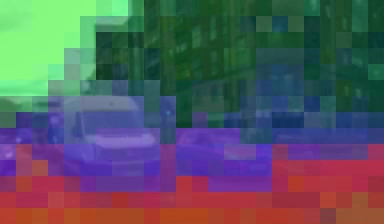
\includegraphics[width=\linewidth]{Figures/Tokenizer/frame1_dino.png}
  \caption{DINO-distilled tokens}
  \label{fig:tokenizer_c}
\end{subfigure}
\caption{Increasing semantic content of image tokens through DINO distillation. Visualization shows the top 3 PCA components of token embeddings mapped to RGB values. DINO-distilled tokens corresponding to a semantic class (e.g. vehicle, road, or sky) have similar embeddings.}
\label{fig:dino_tokenizer}
\end{figure}


%Please refer to \Cref{appendix:image-tokenizer} for a complete description of the image tokenizer.

\subsection{World Model}
\label{subsection:world-model}
As described in \Cref{subsection:encoding} the input of the world model is $(\rvc_1,\rvz_1, \rva_1, ..., \rvc_T, \rvz_T, \rva_T)$. The world model is an autoregressive transformer network that models the sequence input. Its training objective is to predict the next image token in the sequence conditioned on all past tokens, using causal masking in the attention matrix of the transformer blocks \citep{vaswani17}.

\begin{equation}
L_{\text{world model}} = -\sum_{t=1}^T \sum_{i=1}^n\log p(z_{t,i} | \rvz_{<t}, z_{t, j < i}, \rvc_{\leq t}, \rva_{<t})
\end{equation}

We randomly dropout conditioning tokens during training so that the world model can do (i) unconditional generation, (ii) action-conditioned generation, and (iii) text-conditioned generation.

To further reduce the sequence length of our world model we temporally subsample videos from 25Hz to 6.25Hz. This allows the world model to reason over longer periods without leading to intractable sequence lengths. To recover video predictions at full frame rate we perform temporal super-resolution using the video decoder described in \Cref{subsection:video-decoder}.

%A full description of the world model network architecture is given in \Cref{appendix:world-model}.

\subsection{Video Decoder}
\label{subsection:video-decoder}
Following the recent advances in image \citep{rombach2022highresolution, saharia2022photorealistic} and video generation \citep{ho2022imagen, esser2023structure} we use denoising video diffusion models for the GAIA-1 decoder. A naive approach of independently decoding each frame-tokens to pixel space results in a temporally inconsistent video output. Modeling the problem as denoising a sequence of frames during the diffusion process, where the model can access information across time, greatly improves temporal consistency of the output video. 

We follow \citep{ho2022video} and use a 3D U-Net with factorized spatial and temporal attention layers. During training, our video diffusion model is conditioned on the image tokens obtained by discretizing input images with the pre-trained image tokenizer $E_{\theta}$. During inference, the diffusion model is conditioned on the predicted image tokens from the world model.

We train a single model jointly on both image and video generation tasks. Training on videos teaches the decoder to be temporally consistent, while training on images is crucial for the quality of individual frames \citep{ho2022imagen} as it teaches the model to extract information from conditioning image tokens. We disable temporal layers when training on images.

To train our video diffusion decoder for multiple inference tasks we take inspiration from \citep{harvey2022flexible} where we can perform multiple tasks by masking certain frames or the conditioning image tokens. We choose to train a single video diffusion model for all tasks as it has been shown that multi-task training improves performance on individual tasks \citep{harvey2022flexible}. The tasks include image generation, video generation, autoregressive decoding, and video interpolation. Each task is sampled equally. For example, for the autoregressive generation task, we provide previously generated past frames as context and conditioning image tokens for frames we want to predict. We include both forward and backward autoregressive tasks. See \Cref{fig:decoder-tasks} for examples of each task. 
We also apply a conditioning dropout by randomly masking out each conditioning image token with probability $p=0.15$ as it helps the model generalize beyond relying on tokens for information and improves temporal consistency.

\begin{figure}
\centering
\begin{tabular}{cc}
\subfloat[Image generation]{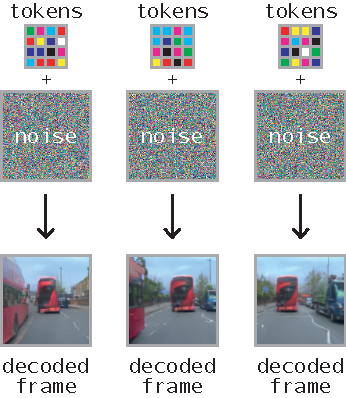
\includegraphics[width = 1.75in]{Figures/Video_Decoder/image_gen.pdf}} \hspace{30pt} &
\subfloat[Video generation]{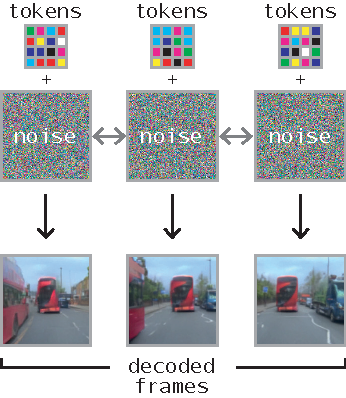
\includegraphics[width = 1.75in]{Figures/Video_Decoder/video_gen.pdf}} \\ [30pt] 
\subfloat[Autoregressive video generation]{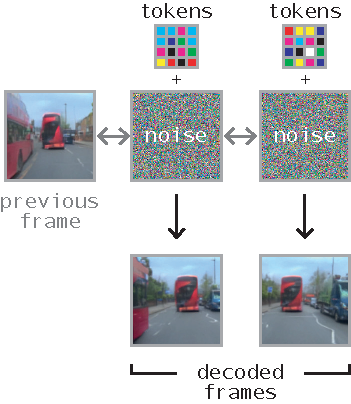
\includegraphics[width = 1.75in]{Figures/Video_Decoder/video_gen_ar.pdf}} \hspace{30pt} &
\subfloat[Video interpolation]{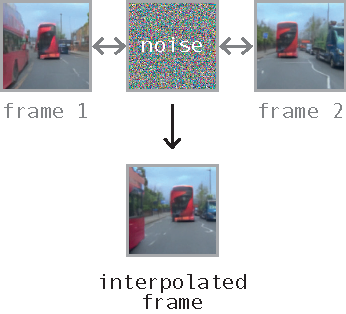
\includegraphics[width = 1.75in]{Figures/Video_Decoder/frame_interp.pdf}}
\end{tabular}
\caption{Video decoder training tasks. Each task is defined by masking ground truth images and context tokens. We pass noise as input for frames we want to predict. Tokens are provided for predicted frames except for video interpolation task where the diffusion process is guided solely by image context.}
\label{fig:decoder-tasks}
\end{figure}

The video decoder is trained on the noise prediction objective. More specifically, we use the $\rvv$-parameterization as proposed in \citep{salimans22} because it avoided unnatural color shifts and maintained long-term consistency as similarly found in \citep{ho2022imagen}. In practice, we use a weighted average of $L_1$ and $L_2$ losses. The video decoder loss $L_{\text{video}}$ is:

\begin{equation}
\label{eq:diffusion-loss}
L_{\text{video}}= \mathbb{E}_{\mathbf{\epsilon}, t'} \left[\lVert 
\mathbf{\epsilon}_{\theta}(\rvx^{t'}, t', \rvz, \rvm)
-
\mathbf{\epsilon}
\rVert^2_2 \right]
\end{equation}

where:
\begin{itemize}
\item $\mathbf{\epsilon}_\mathbf{\theta}$ is the denoising video model.
\item $\epsilon$ is the denoising target, which uses the $\rvv$-parameterization.
\item $t' \sim U(0,1)$ is the sampled discrete diffusion time.
\item $\rvx=(\rvx_1, ..., \rvx_{T'})$ is a video sequence of length $T'$.
\item $\rvx^{t'} = \alpha_{t'}\mathbf{x} + \sigma_{t'}\mathbf{\epsilon}$ represents the noised video, with $\alpha_{t'}$ and $\sigma_{t'}$ functions of $t'$ that define the noise schedule.
\item $\rvz=(\rvz_1, ..., \rvz_{T'}) = E_{\theta}(\rvx)$ is the sequence of conditioning image tokens.
\item $\rvm=(\rvm_1, ..., \rvm_{T'})$ is a sequence of image masks as specified by the training task (see \Cref{fig:decoder-tasks}).
\end{itemize}

%For a full description of decoder architecture, please refer to \Cref{appendix:video-decoder}.


